\section{Analyse des paramètres des fonctions de magnitude}
\subsection{Analyse de $m_1(x,y)$}
\begin{figure}[!h]
   \begin{subfigure}[c]{.5\linewidth}
     \centering
     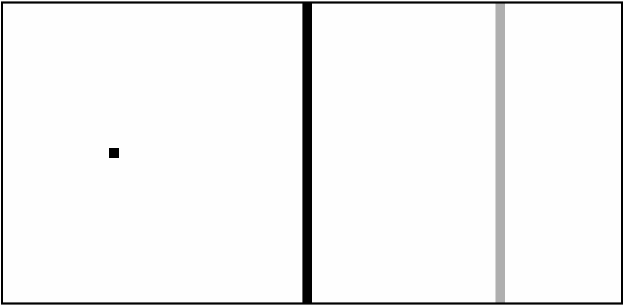
\includegraphics[scale=0.35]{Chapters/Images/synthetic_map.png}
     \caption{}
   \end{subfigure} 
   \begin{subfigure}[c]{.5\linewidth}
     \centering
     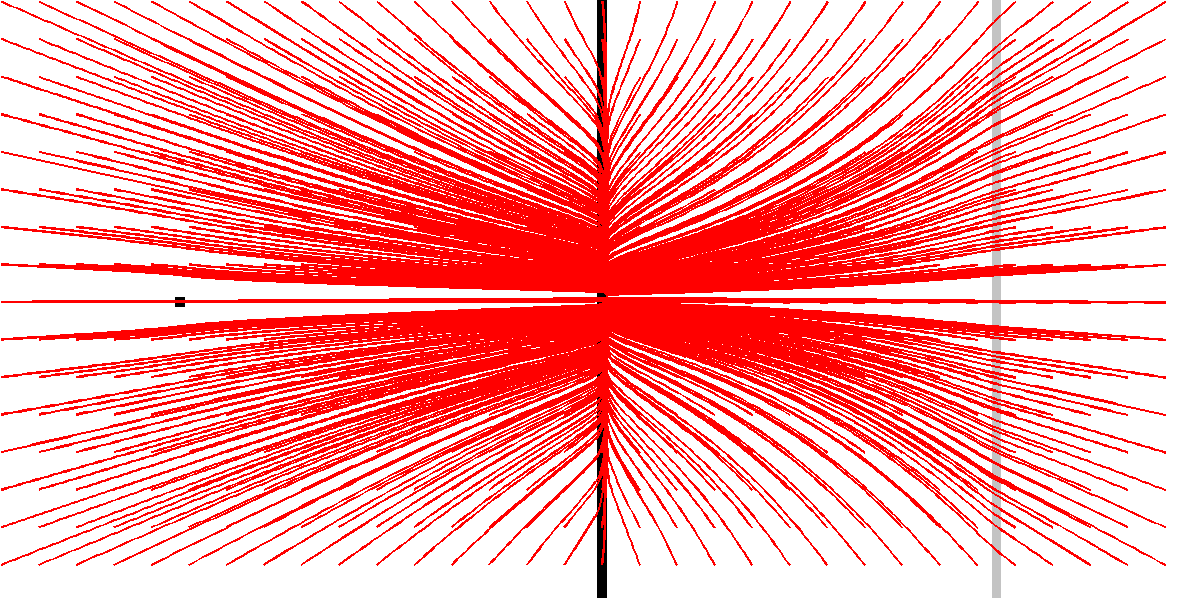
\includegraphics[scale=0.35]{Chapters/Images/m1_gamma_5.png}
     \caption{$\gamma=0.5$}
   \end{subfigure} \\
   
   \begin{subfigure}[c]{.5\linewidth}
     \centering
     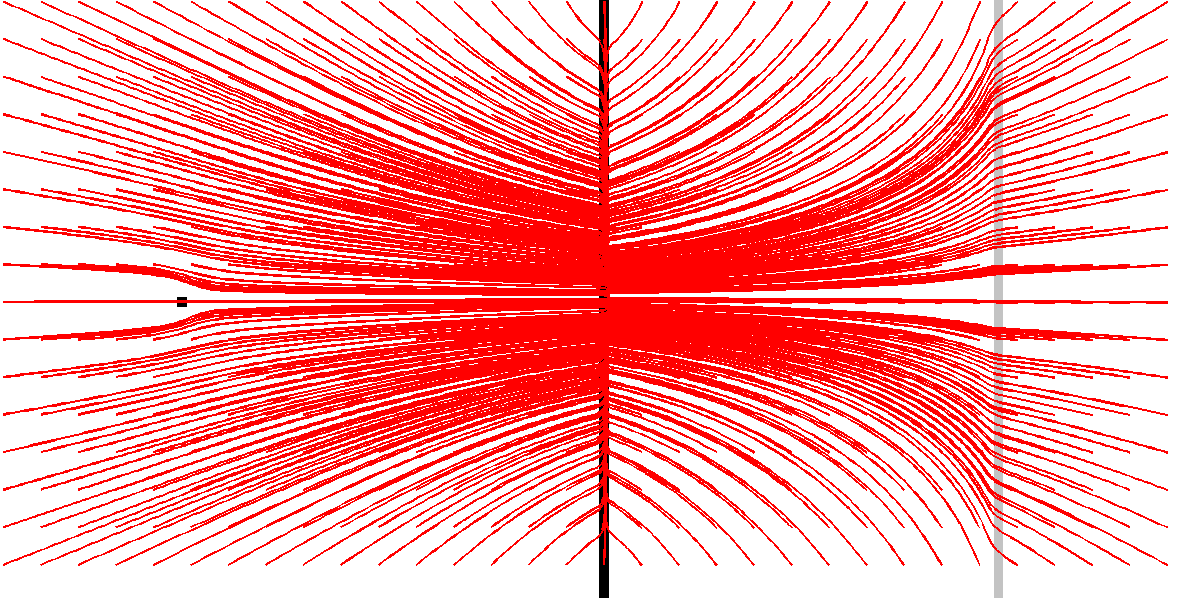
\includegraphics[scale=0.35]{Chapters/Images/m1_gamma_10.png}
     \caption{$\gamma=1.0$}
   \end{subfigure}
   \begin{subfigure}[c]{.5\linewidth}
     \centering
     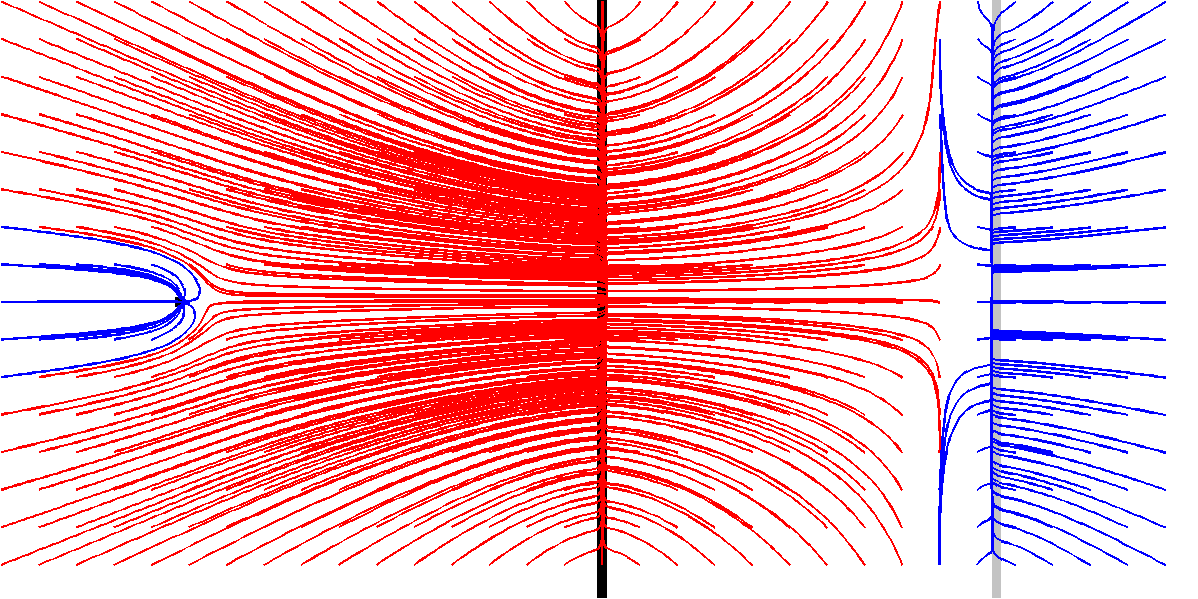
\includegraphics[scale=0.35]{Chapters/Images/m1_gamma_15.png}
     \caption{$\gamma=1.5$}
   \end{subfigure}\\
   
   \begin{subfigure}[c]{.5\linewidth}
     \centering
     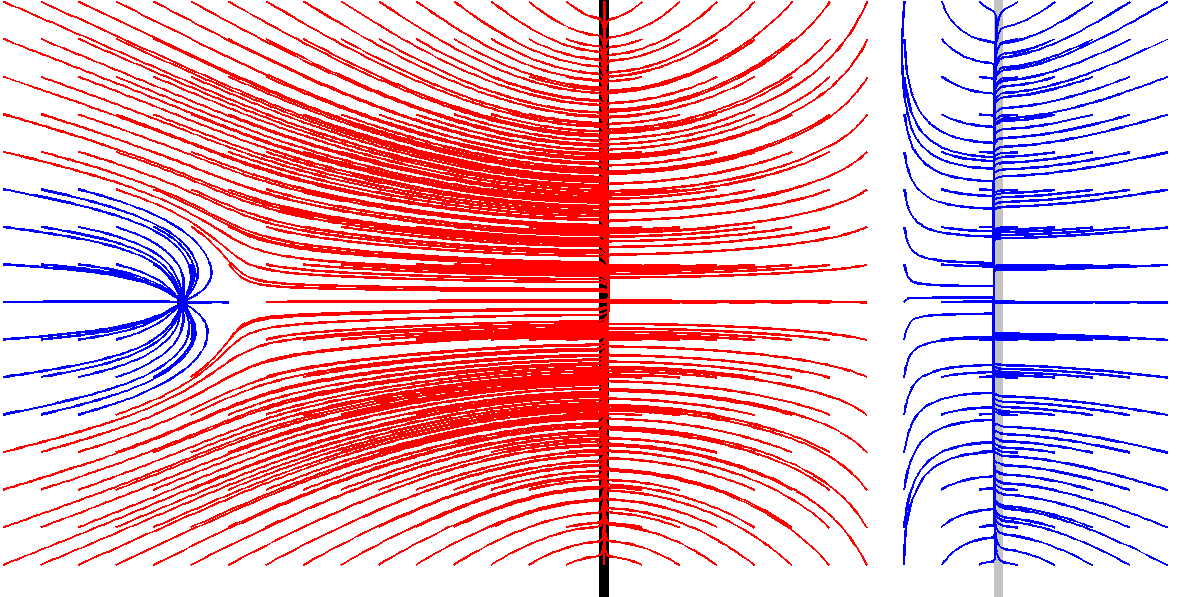
\includegraphics[scale=0.35]{Chapters/Images/m1_gamma_20.png}
     \caption{$\gamma=2.0$}
   \end{subfigure}
   \begin{subfigure}[c]{.5\linewidth}
     \centering
     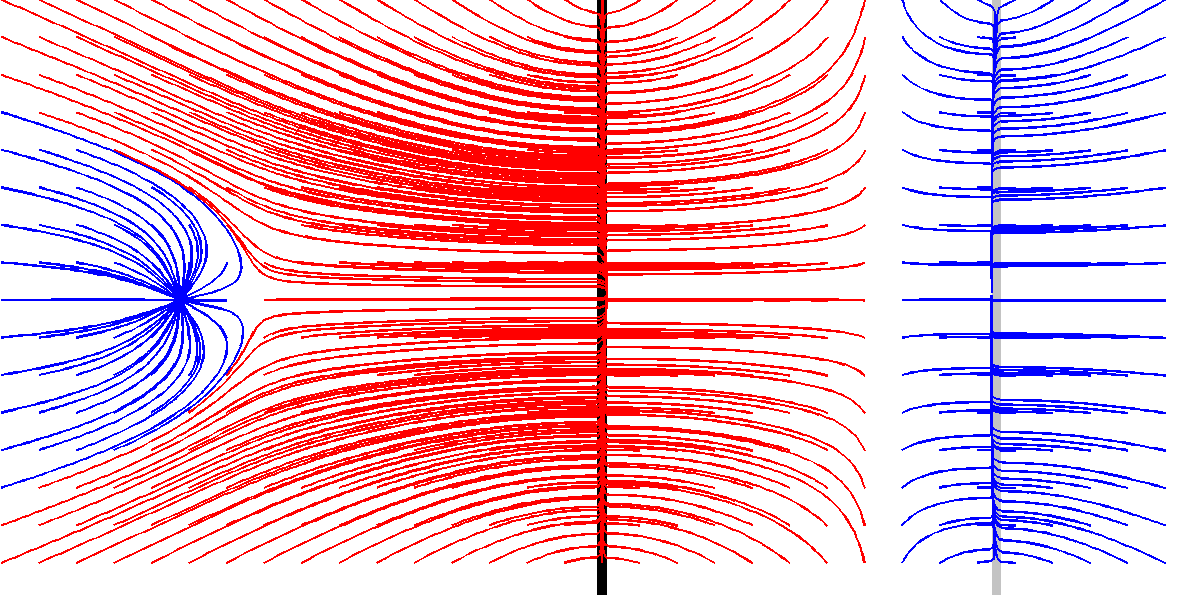
\includegraphics[scale=0.35]{Chapters/Images/m1_gamma_25.png}
     \caption{$\gamma=2.5$}
   \end{subfigure}\\
   
   \caption{(a) Carte de contours $F(x,y)$ synthétique avec un bruit impulsionnel, un contour fort et un contour faible. Lignes de courant générées à partir du champ VFC utilisant $m_1(x,y)$ avec plusieurs valeurs du paramètre $\gamma$ et pour un rayon $R=128$ du noyau de convolution.}
   \label{fig:gamma}
\end{figure}
\subsection{Analyse de $m_1(x,y)$}
\begin{figure}[!h]
   \begin{subfigure}[c]{.5\linewidth}
     \centering
     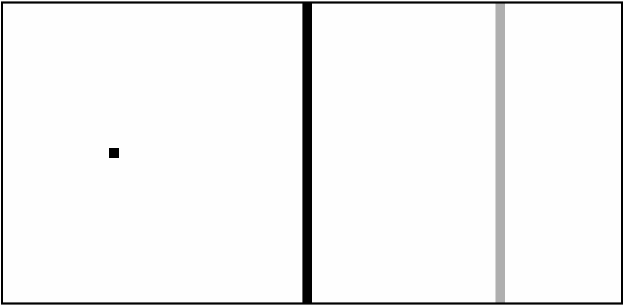
\includegraphics[width=\textwidth]{Chapters/Images/synthetic_map.png}
     \caption{}
   \end{subfigure} 
      \begin{subfigure}[c]{.5\linewidth}
     \centering
     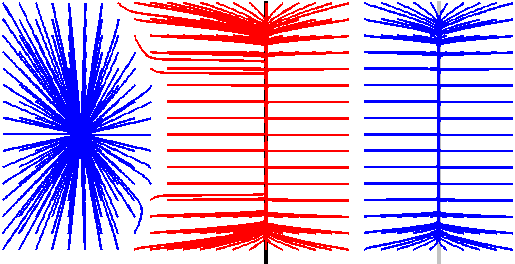
\includegraphics[width=\textwidth]{Chapters/Images/m2_sigma_10.png}
     \caption{$\sigma=10$}
   \end{subfigure} \\
   
   \begin{subfigure}[c]{.5\linewidth}
     \centering
     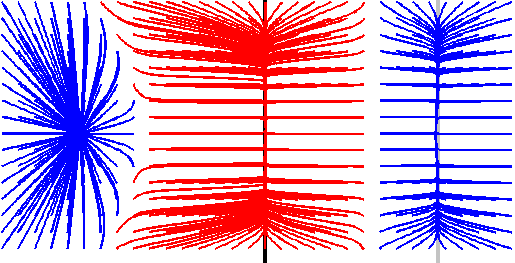
\includegraphics[width=\textwidth]{Chapters/Images/m2_sigma_15.png}
     \caption{$\sigma=15$}
   \end{subfigure}   
   \begin{subfigure}[c]{.5\linewidth}
     \centering
     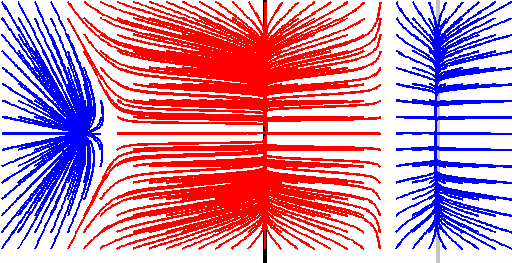
\includegraphics[width=\textwidth]{Chapters/Images/m2_sigma_20.png}
     \caption{$\sigma=20$}
   \end{subfigure}\\
   
   \begin{subfigure}[c]{.5\linewidth}
     \centering
     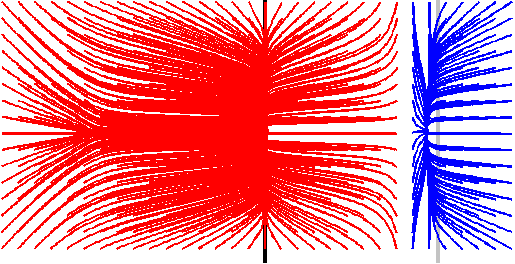
\includegraphics[width=\textwidth]{Chapters/Images/m2_sigma_25.png}
     \caption{$\sigma=25$}
   \end{subfigure}
   \begin{subfigure}[c]{.5\linewidth}
     \centering
     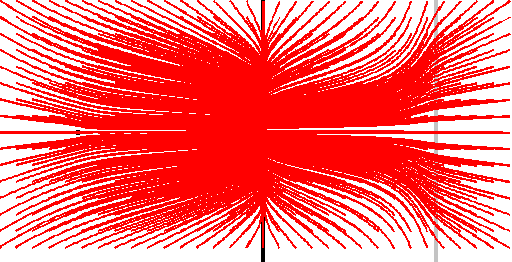
\includegraphics[width=\textwidth]{Chapters/Images/m2_sigma_30.png}
     \caption{$\sigma=30$}
   \end{subfigure}\\
   
   \caption{(a) Carte de contours $F(x,y)$ synthétique avec un bruit impulsionnel, un contour fort et un contour faible. Lignes de courant générées à partir du champ VFC utilisant $m_2(x,y)$ avec plusieurs valeurs du paramètre $\sigma$ et pour un rayon $R=128$ du noyau de convolution.}
   \label{fig:sigma}
\end{figure}

\section{Analyse de la convergence dans les zones concaves}
\label{ann_concavities_results}

\begin{figure}[H]
\begin{subfigure}[c]{0.3\linewidth}
\centering
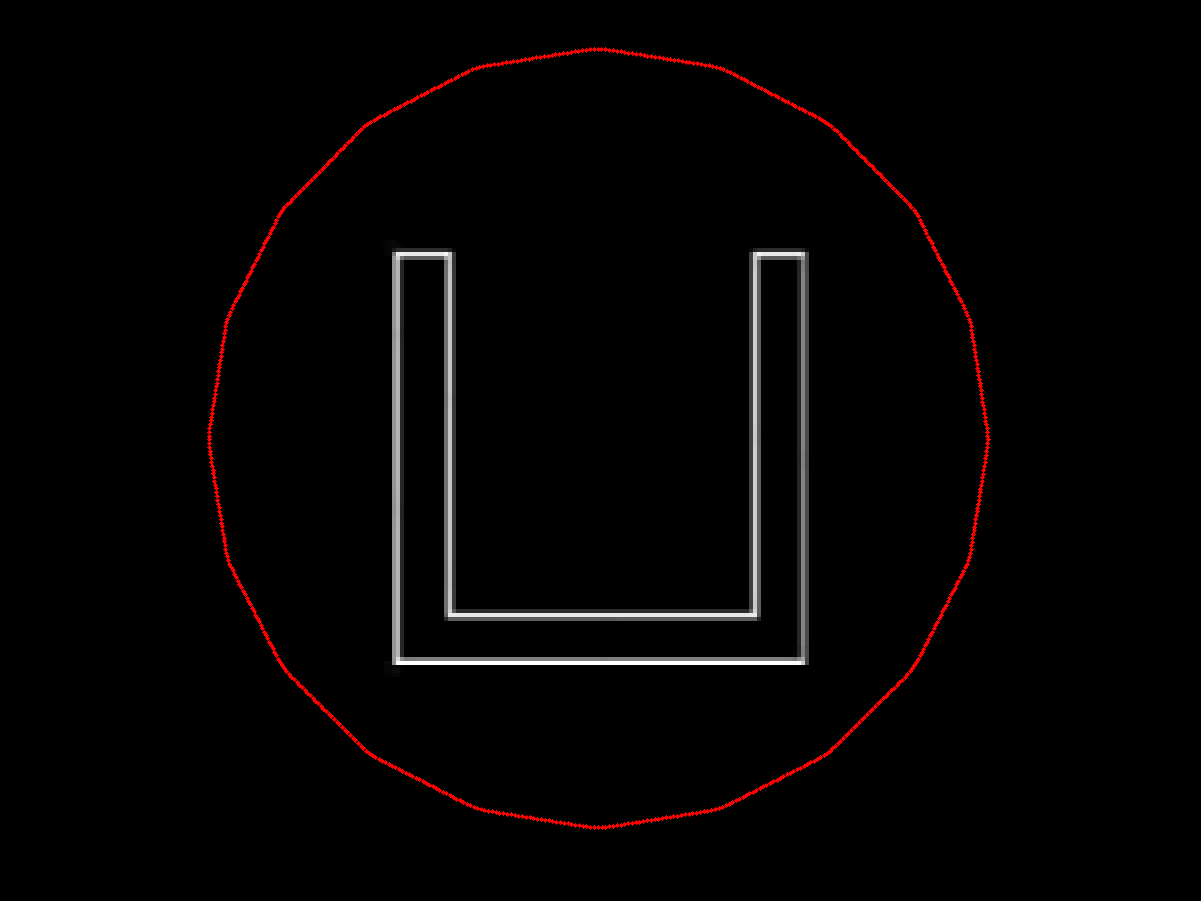
\includegraphics[width=\textwidth]{Chapters/Images/Conc/sq}
\caption{}
\end{subfigure}
\begin{subfigure}[c]{0.3\linewidth}
\centering
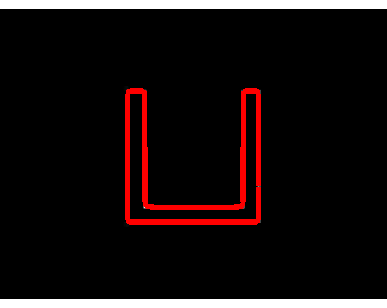
\includegraphics[width=\textwidth]{Chapters/Images/Conc/gvfsq}
\caption{}
\end{subfigure}
\begin{subfigure}[c]{0.3\linewidth}
\centering
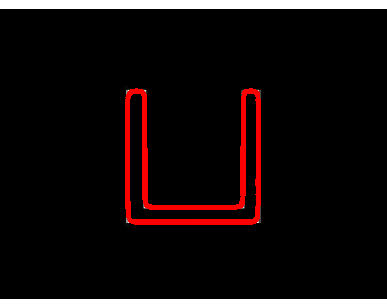
\includegraphics[width=\textwidth]{Chapters/Images/Conc/vfcsq}
\caption{}
\end{subfigure}
\\
\begin{subfigure}[c]{0.3\linewidth}
\centering

\includegraphics[width=\textwidth]{Chapters/Images/Conc/star}
\caption{}
\end{subfigure}
\begin{subfigure}[c]{0.3\linewidth}
\centering
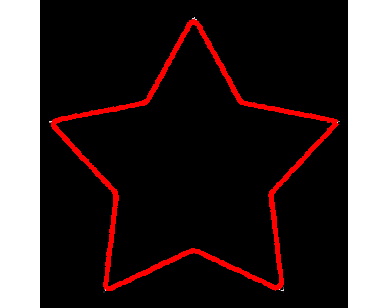
\includegraphics[width=\textwidth]{Chapters/Images/Conc/gvfs}
\caption{}
\end{subfigure}
\begin{subfigure}[c]{0.3\linewidth}
\centering
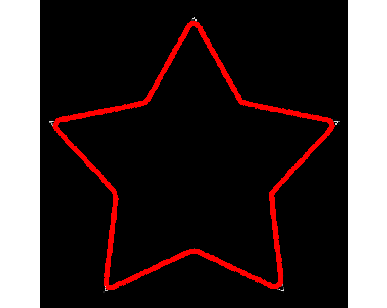
\includegraphics[width=\textwidth]{Chapters/Images/Conc/vfcs}
\caption{}
\end{subfigure}
\caption{(a),(b) : initialisation du contour actif(b),(e) : GVF ($\mu = 0.2$, $nb_{iter} = 10000$), (c), (f) : VCF ($R = 128$, force $m_{1}$ avec $\gamma = 1.7$)}
\end{figure}

\begin{figure}[H]
\centering
\begin{subfigure}[c]{0.4\linewidth}
\centering
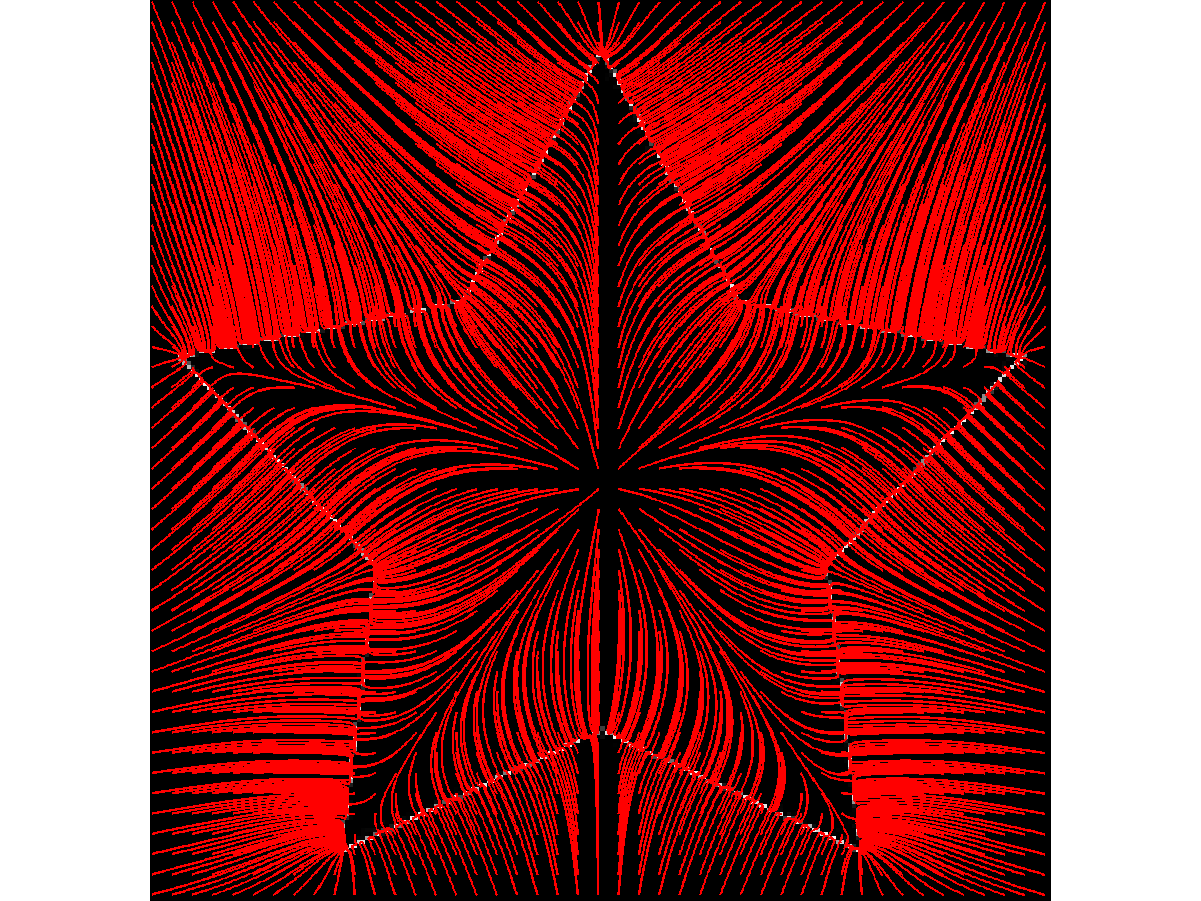
\includegraphics[width=\textwidth]{Chapters/Images/Conc/gvfsstream}
\caption{}
\end{subfigure}
\begin{subfigure}[c]{0.4\linewidth}
\centering
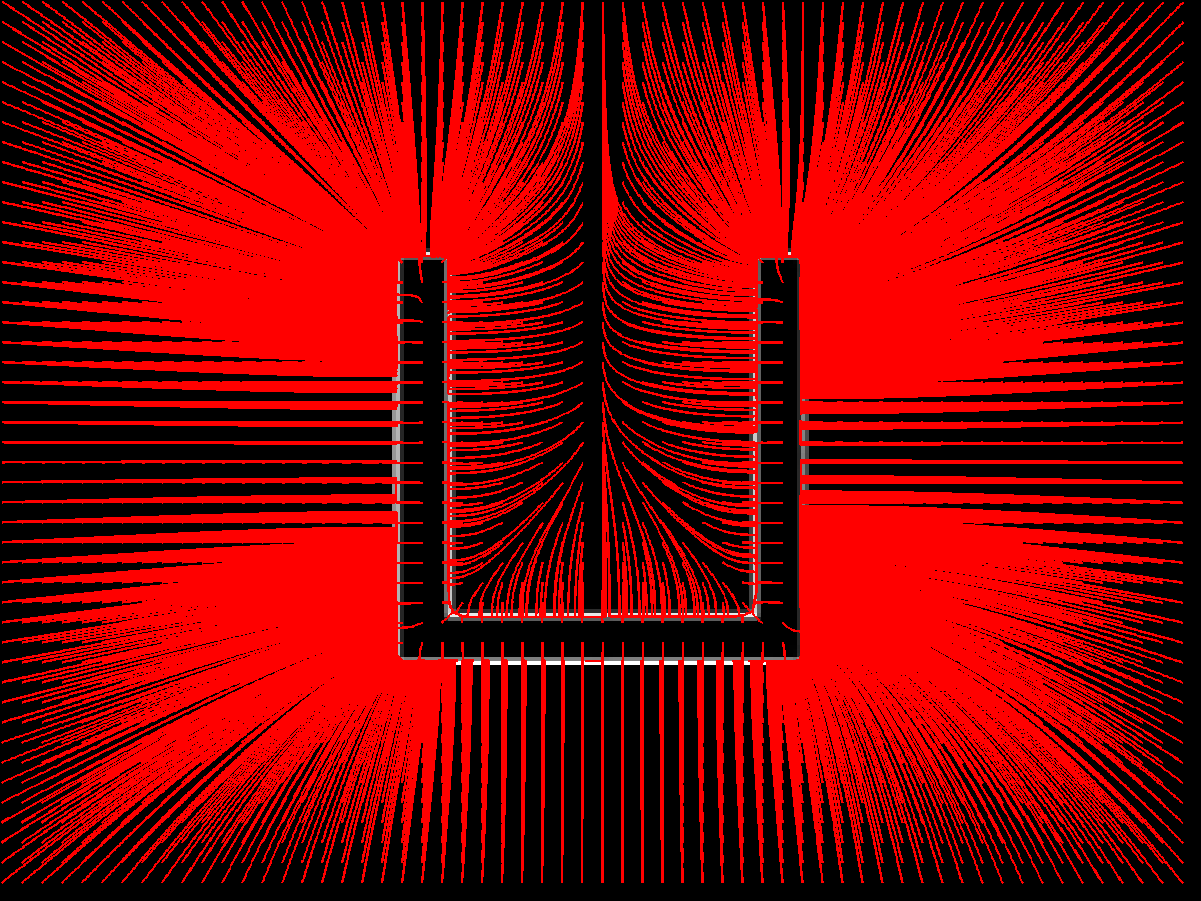
\includegraphics[width=\textwidth]{Chapters/Images/Conc/gvfsqstream}
\caption{}
\end{subfigure}
\\
\begin{subfigure}[c]{0.4\linewidth}
\centering
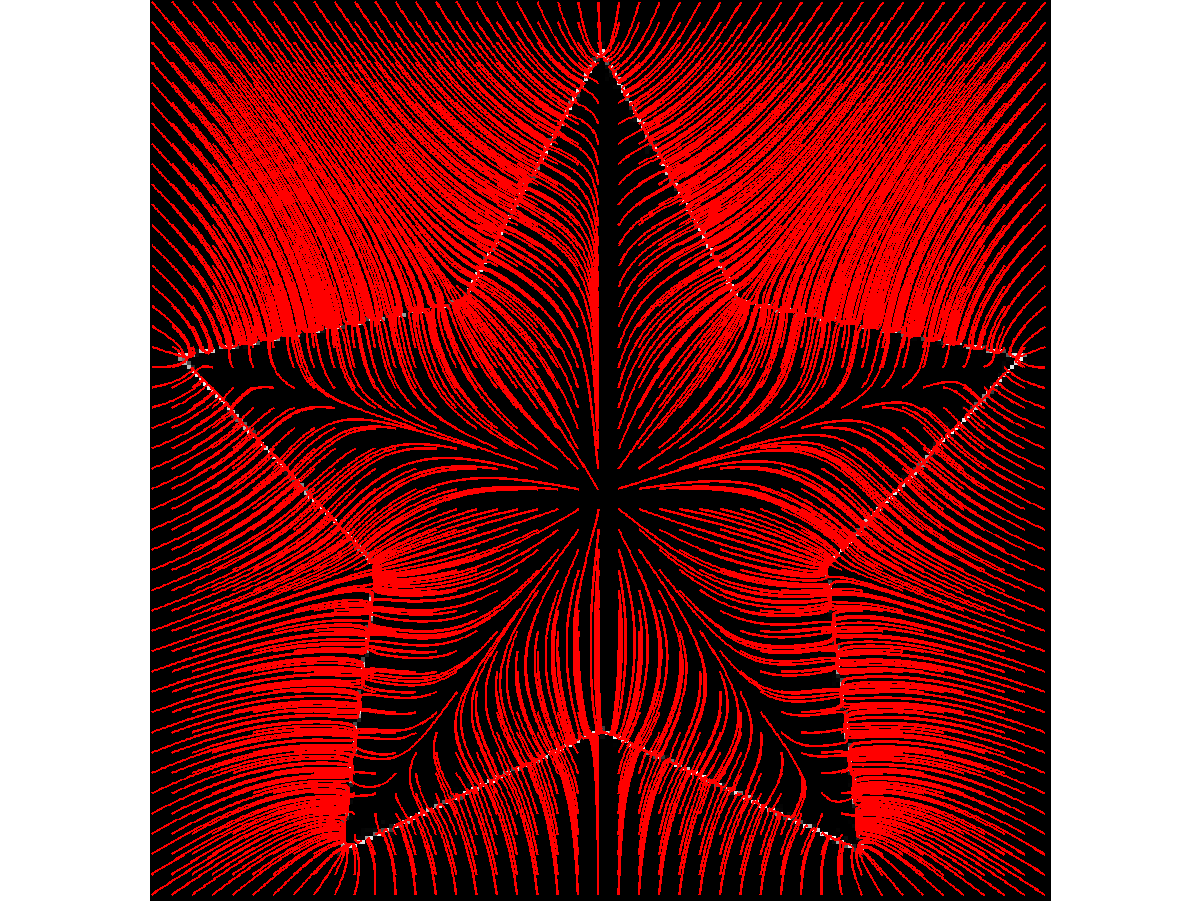
\includegraphics[width=\textwidth]{Chapters/Images/Conc/vfcsstream}
\caption{}
\end{subfigure}
\begin{subfigure}[c]{0.4\linewidth}
\centering
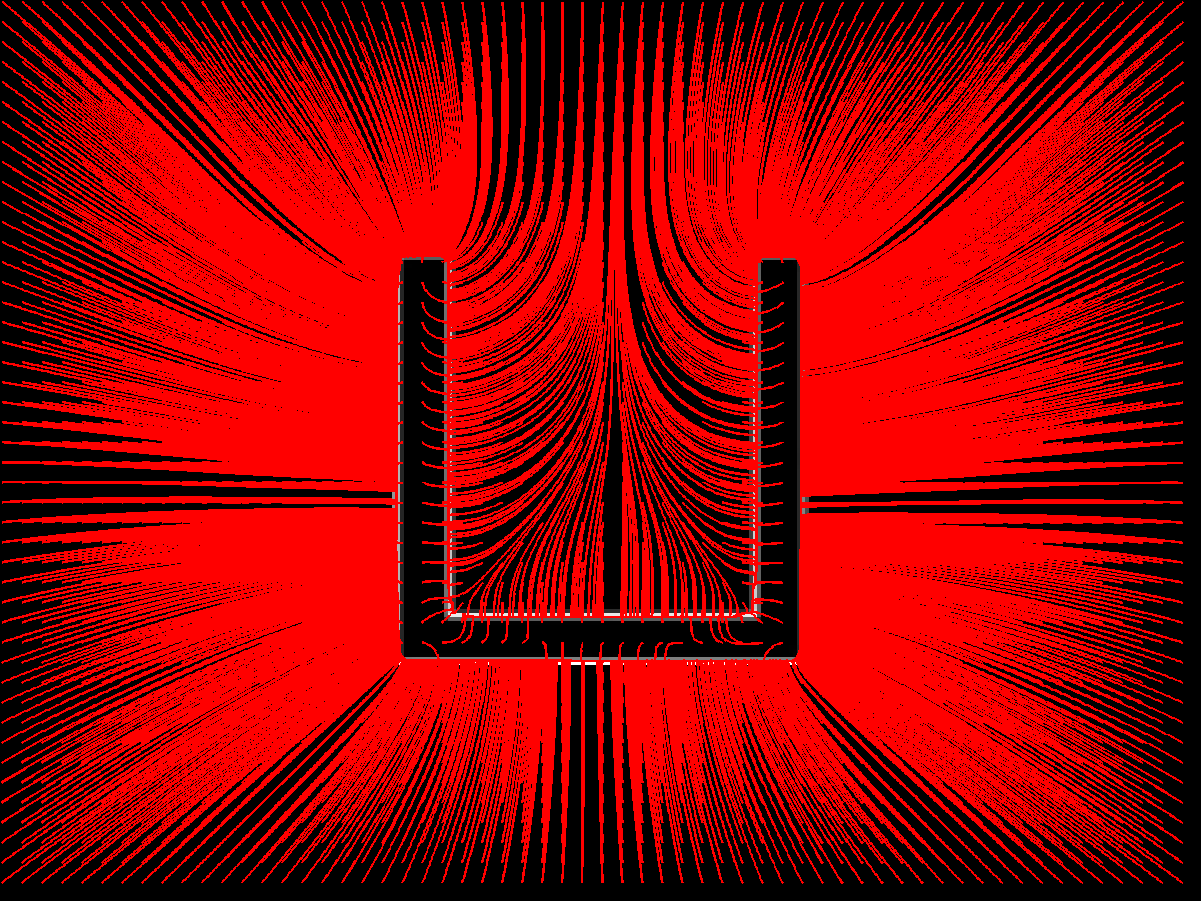
\includegraphics[width=\textwidth]{Chapters/Images/Conc/vfcsqstream}
\caption{}
\end{subfigure}
\caption{(a),(b) : GVF streamlines (c),(d) : VFC streamline}
\end{figure}

\section{Analyse de la robustesse à l'initialisation des contours actifs}
\label{ann_init_results}

\begin{figure}[H]
\begin{subfigure}[c]{0.3\linewidth}
\centering
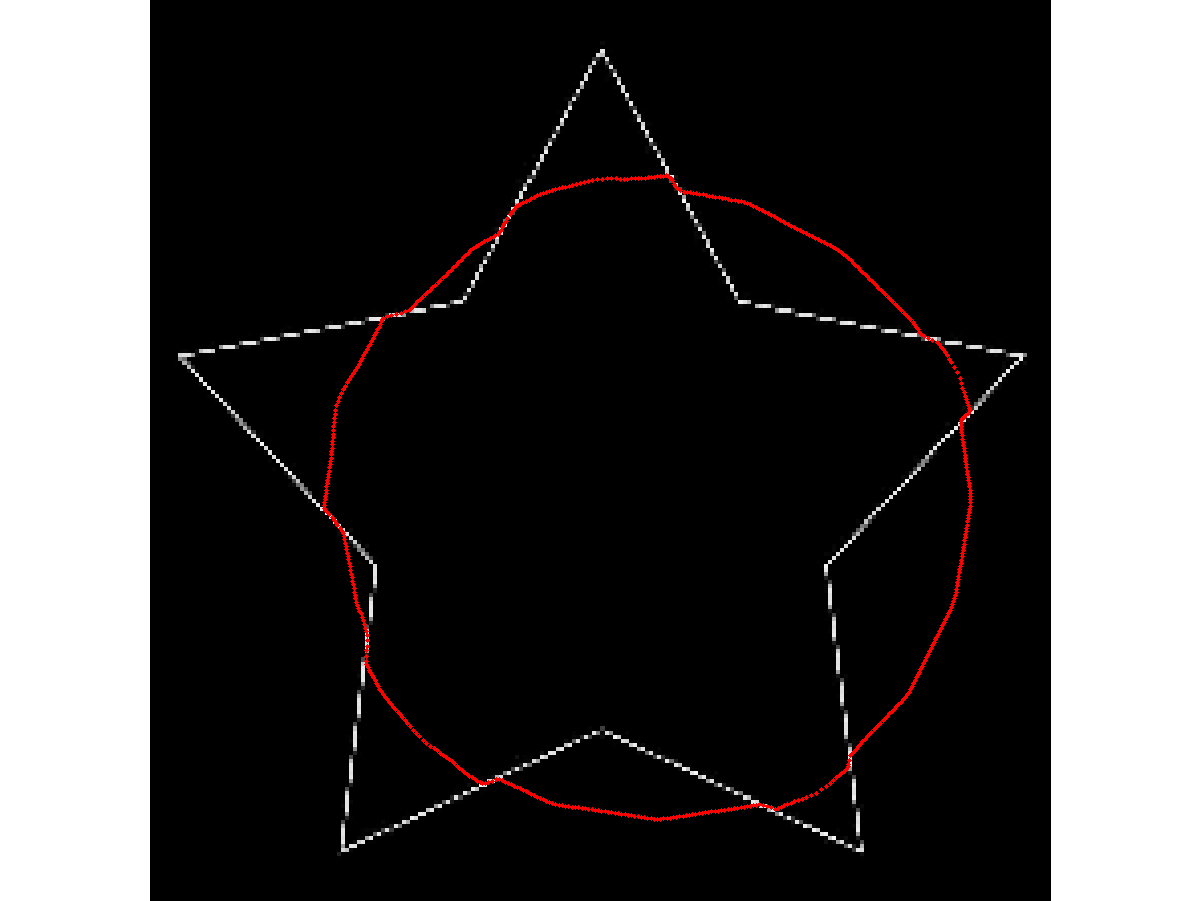
\includegraphics[width=\textwidth]{Chapters/Images/Init/vfccl1}
\caption{}
\end{subfigure}
\begin{subfigure}[c]{0.3\linewidth}
\centering
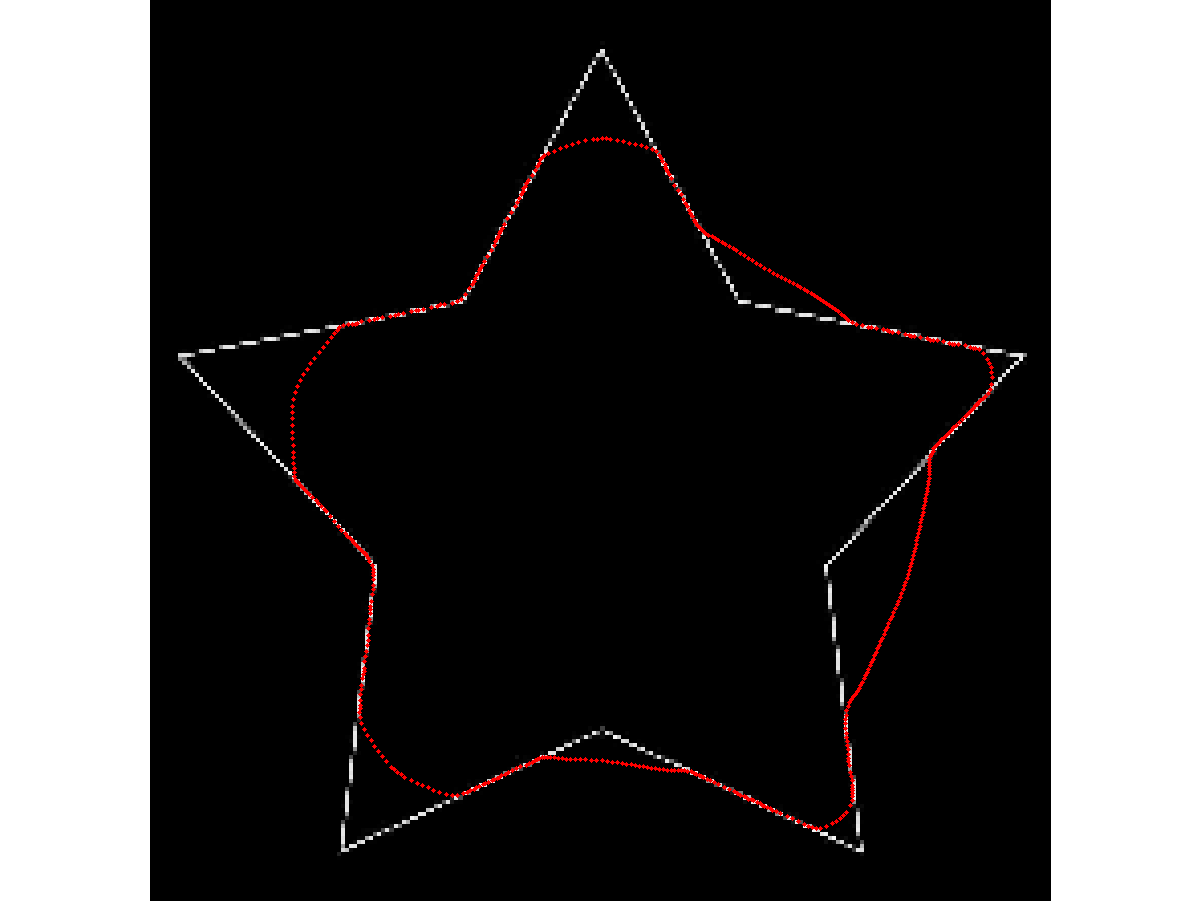
\includegraphics[width=\textwidth]{Chapters/Images/Init/vfccl2}
\caption{}
\end{subfigure}
\begin{subfigure}[c]{0.3\linewidth}
\centering
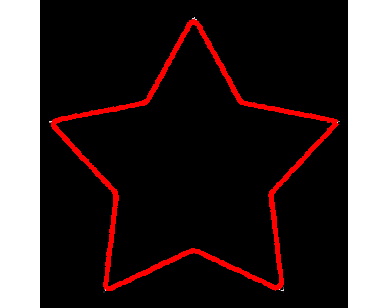
\includegraphics[width=\textwidth]{Chapters/Images/Init/vfccl3}
\caption{}
\end{subfigure}
\caption{Initialisation centrée et taille importante - Convergence vers l'objet d'intérêt}
\end{figure}

\begin{figure}[H]
\begin{subfigure}[c]{0.3\linewidth}
\centering
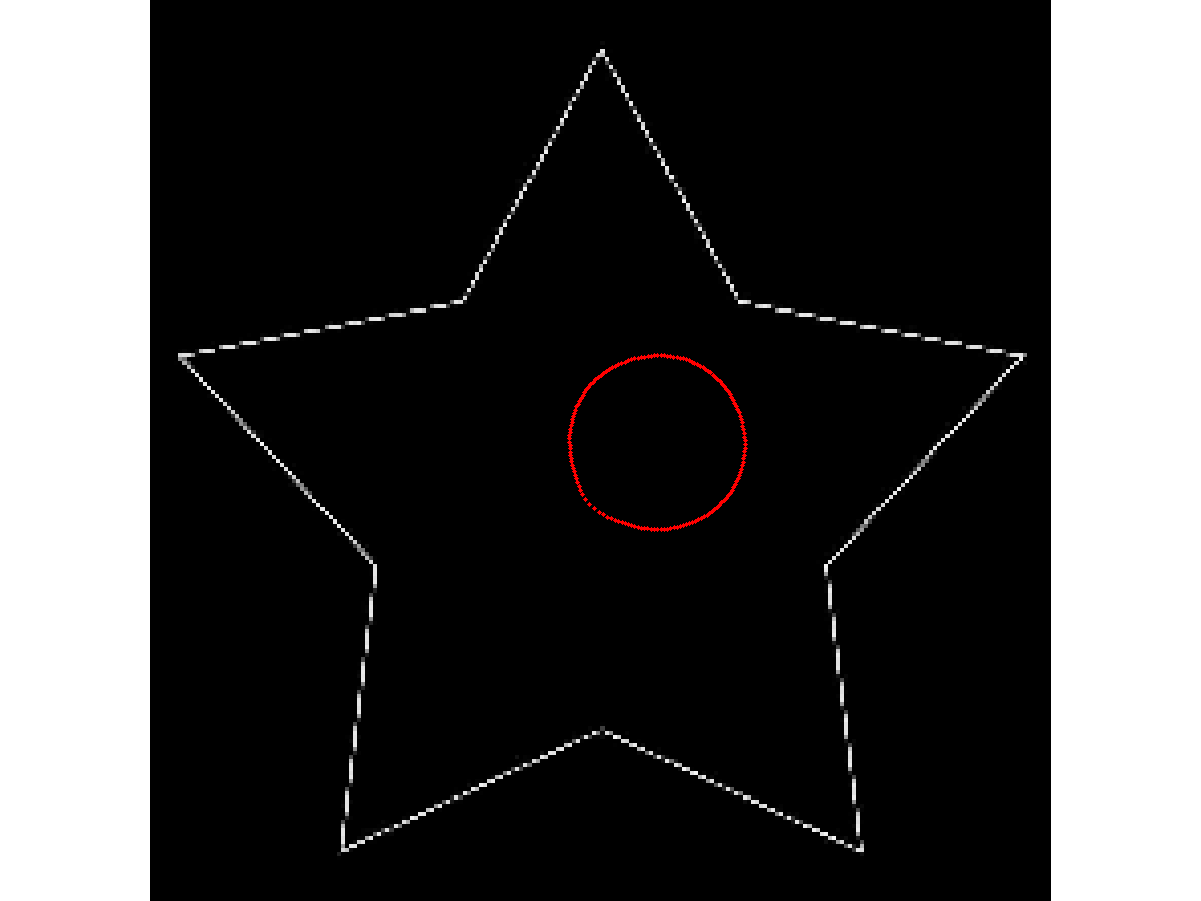
\includegraphics[width=\textwidth]{Chapters/Images/Init/vfccs1}
\caption{}
\end{subfigure}
\begin{subfigure}[c]{0.3\linewidth}
\centering
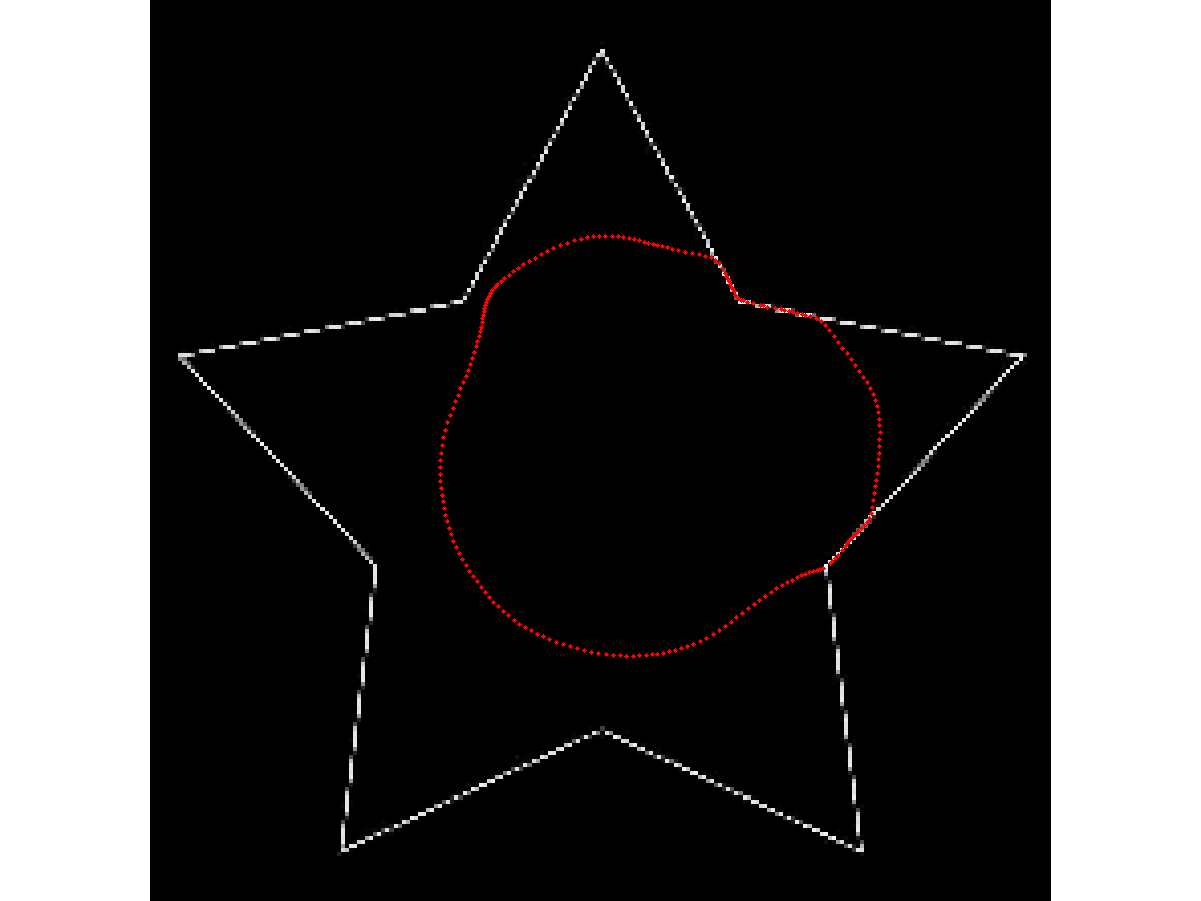
\includegraphics[width=\textwidth]{Chapters/Images/Init/vfccs2}
\caption{}
\end{subfigure}
\begin{subfigure}[c]{0.3\linewidth}
\centering
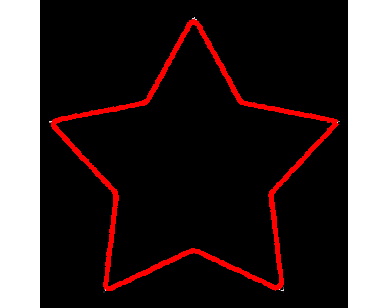
\includegraphics[width=\textwidth]{Chapters/Images/Init/vfccs3}
\caption{}
\end{subfigure}
\caption{Initialisation centrée et petite taille - Convergence vers l'objet d'intérêt}
\end{figure}

\begin{figure}[H]
\begin{subfigure}[c]{0.3\linewidth}
\centering
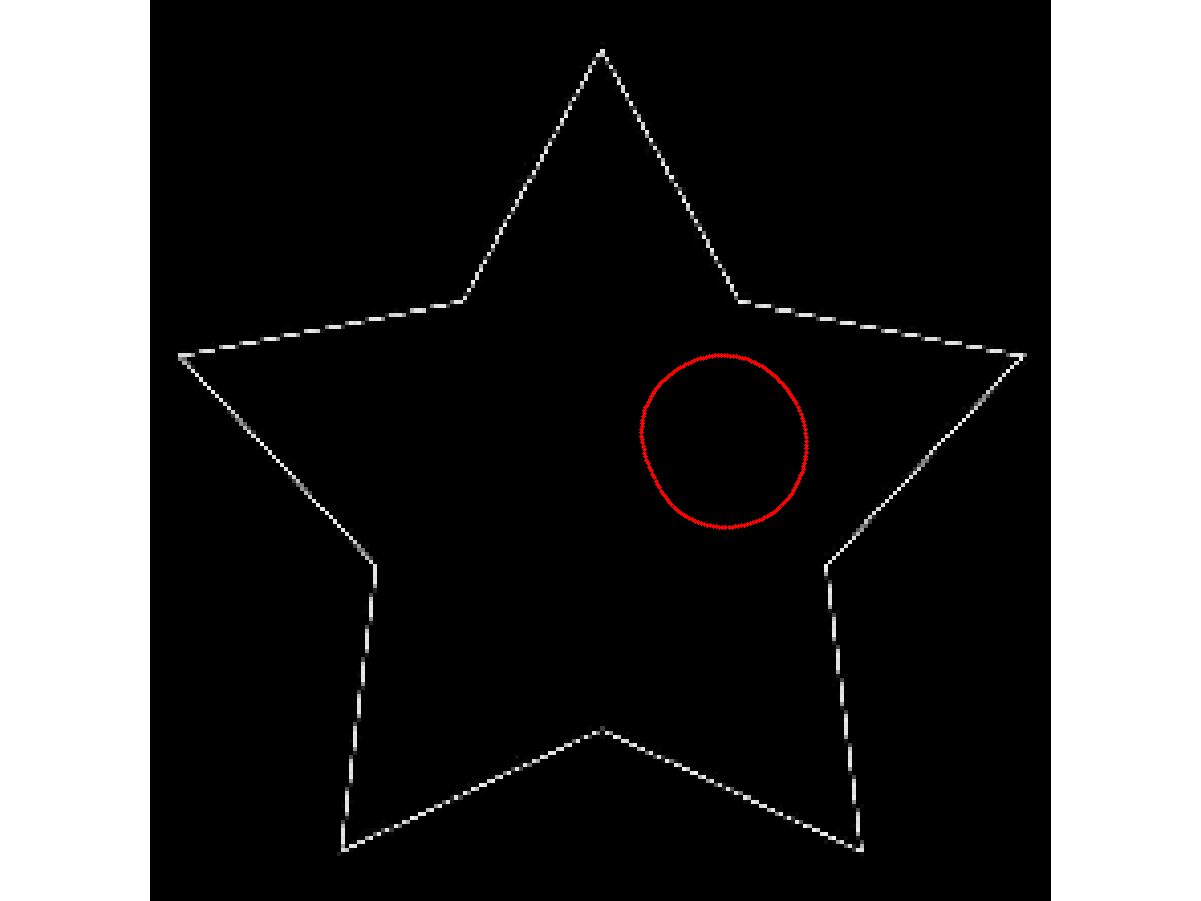
\includegraphics[width=\textwidth]{Chapters/Images/Init/vfcus1}
\caption{}
\end{subfigure}
\begin{subfigure}[c]{0.3\linewidth}
\centering
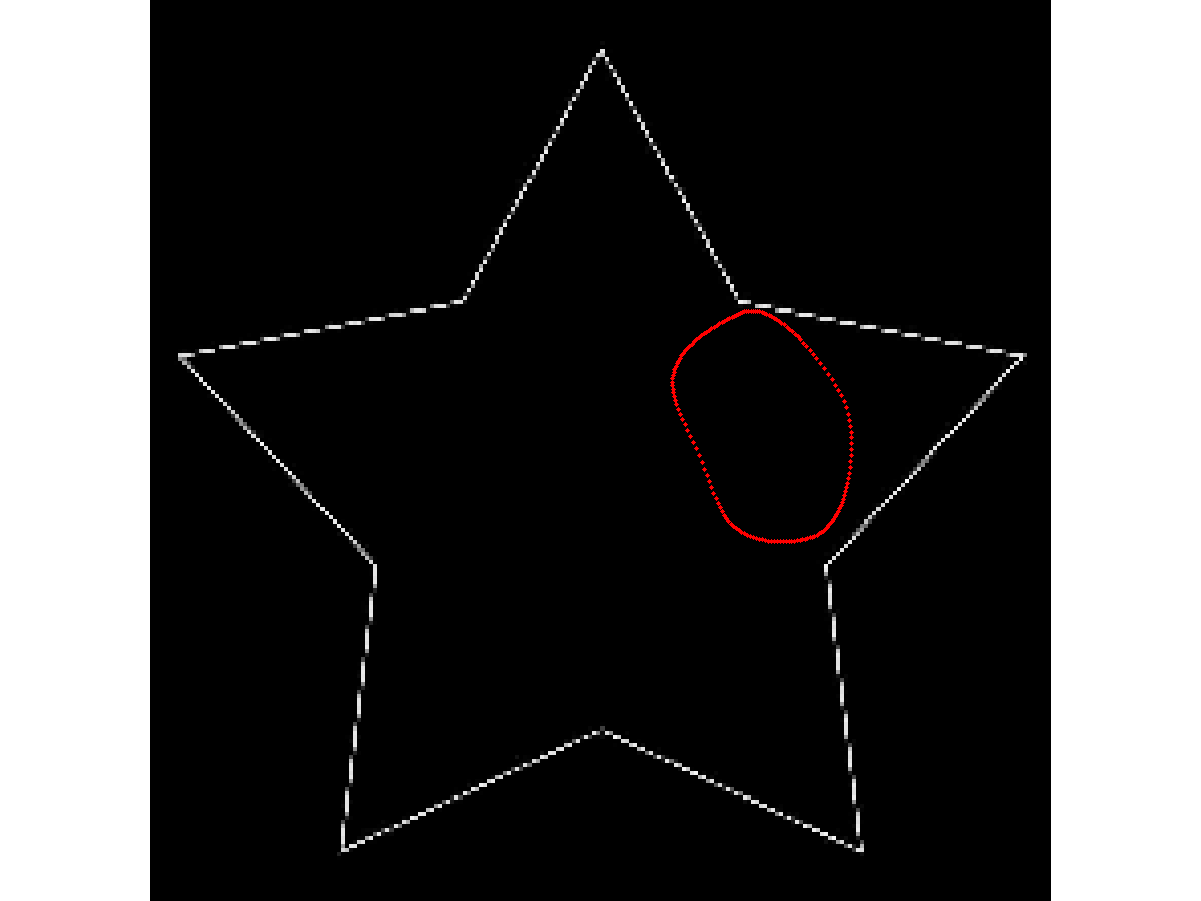
\includegraphics[width=\textwidth]{Chapters/Images/Init/vfcus2}
\caption{}
\end{subfigure}
\begin{subfigure}[c]{0.3\linewidth}
\centering
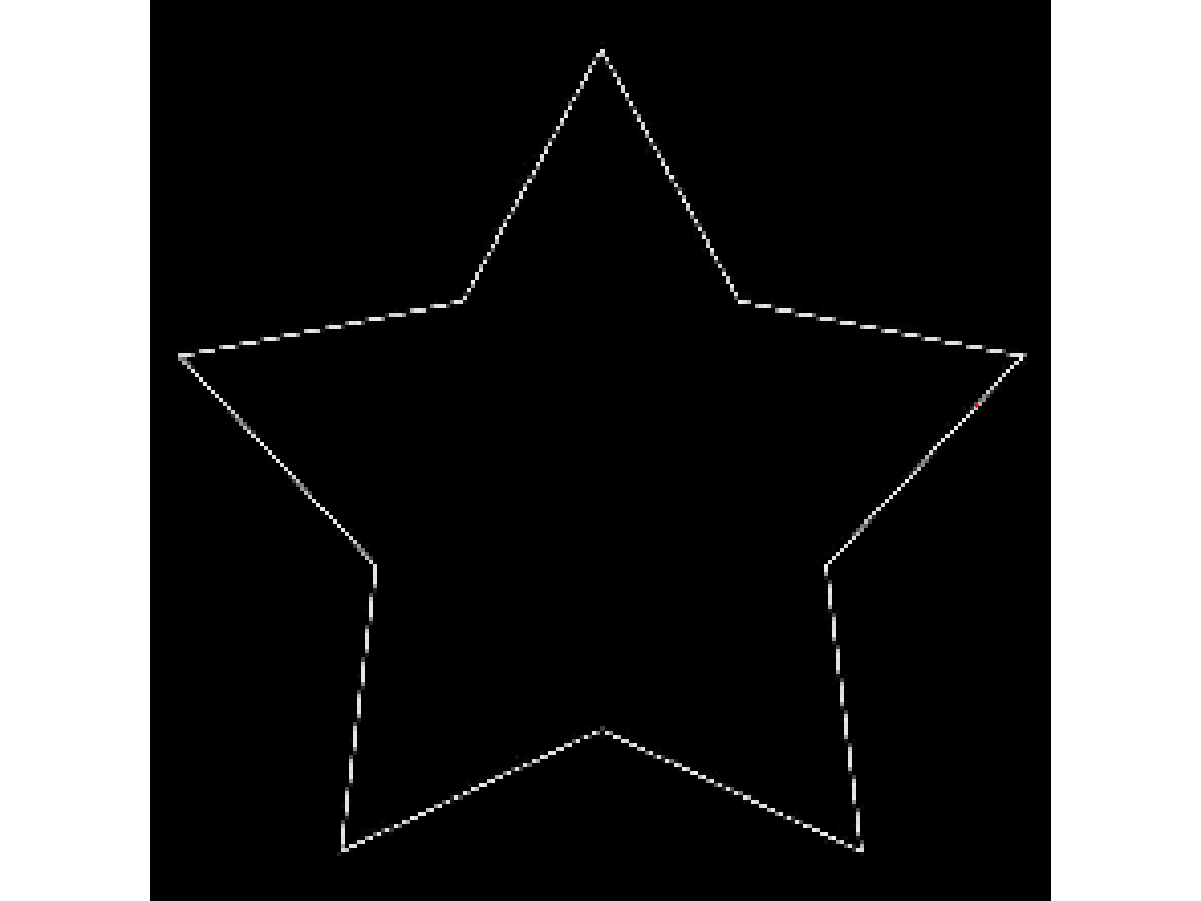
\includegraphics[width=\textwidth]{Chapters/Images/Init/vfcus3}
\caption{}
\end{subfigure}
\caption{Initialisation non centrée et petite taille - Pas de convergence vers l'objet d'intérêt}
\end{figure}

\begin{figure}[H]
\begin{subfigure}[c]{0.3\linewidth}
\centering
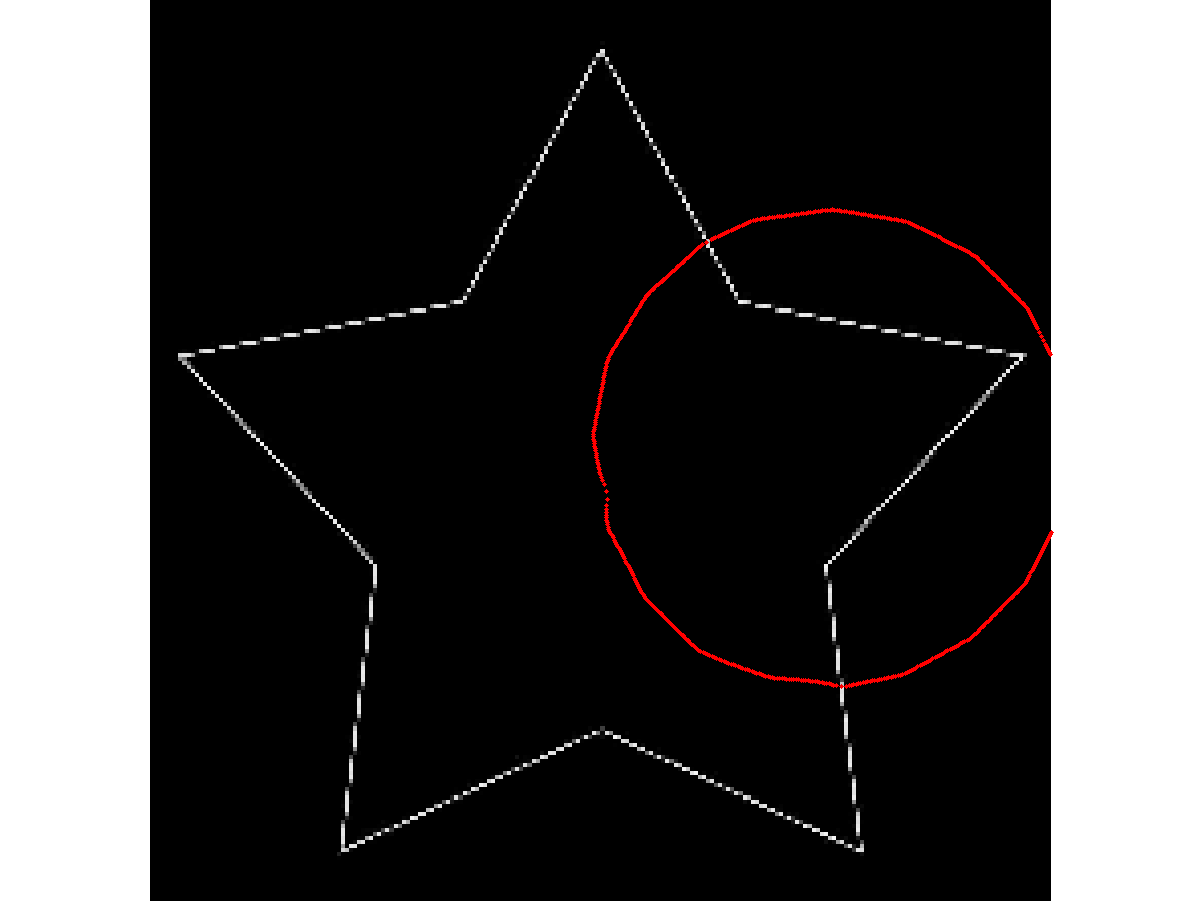
\includegraphics[width=\textwidth]{Chapters/Images/Init/vfcusym1}
\caption{}
\end{subfigure}
\begin{subfigure}[c]{0.3\linewidth}
\centering
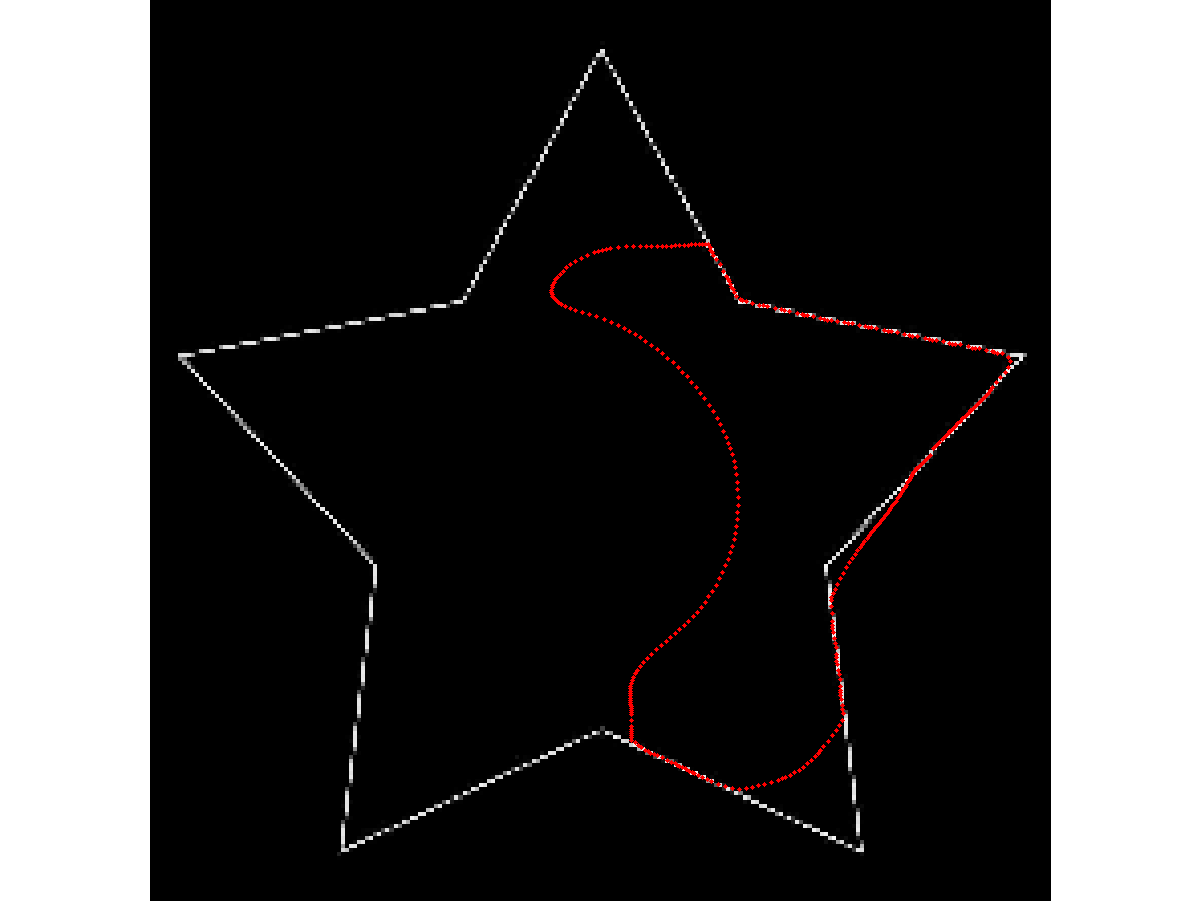
\includegraphics[width=\textwidth]{Chapters/Images/Init/vfcusym2}
\caption{}
\end{subfigure}
\begin{subfigure}[c]{0.3\linewidth}
\centering
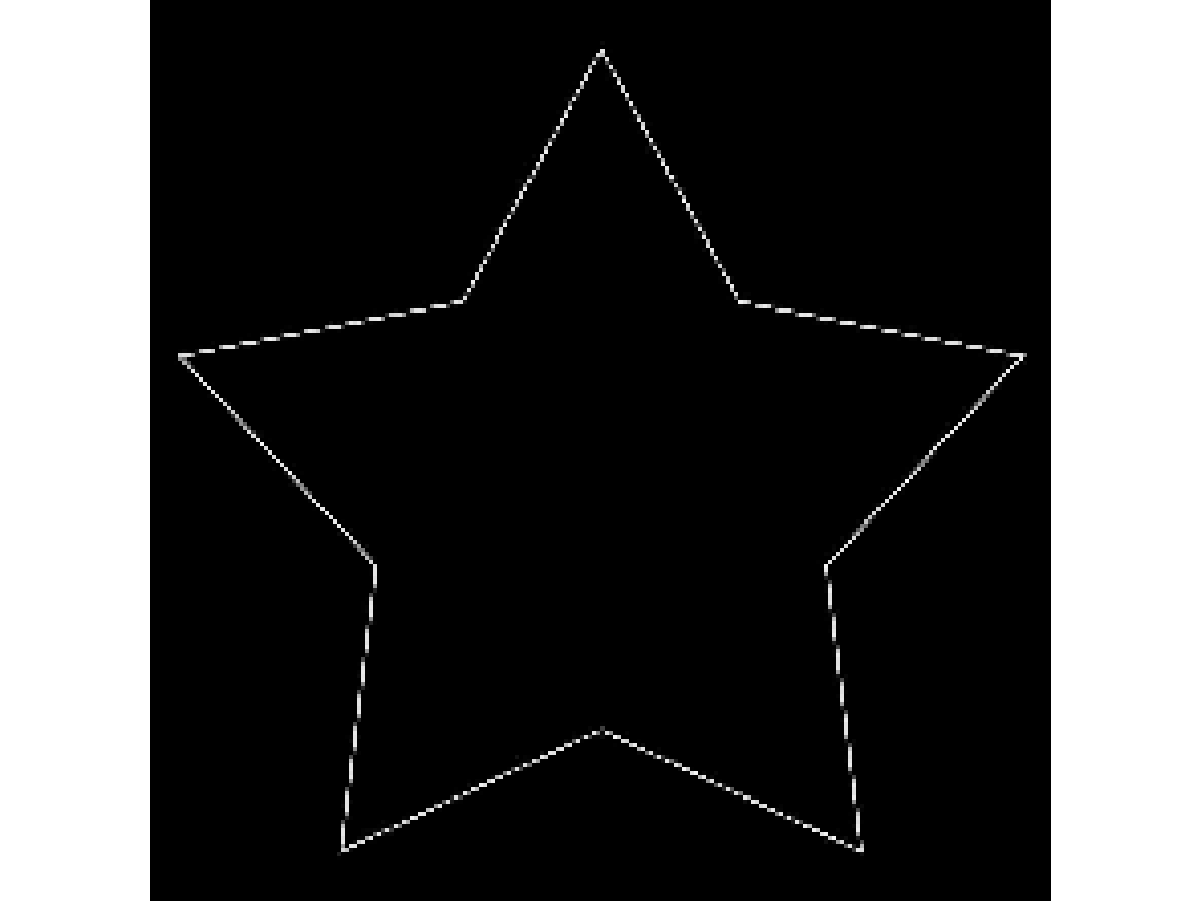
\includegraphics[width=\textwidth]{Chapters/Images/Init/vfcusym3}
\caption{}
\end{subfigure}
\caption{Initialisation non centrée mais se rapprochant du centre de symétrie - Pas de convergence vers l'objet d'intérêt}
\end{figure}

\section{Analyse de la robustesse au bruit}
\label{ann_noise_results}

\begin{figure}[H]
\centering
\begin{subfigure}[c]{0.3\linewidth}
\centering
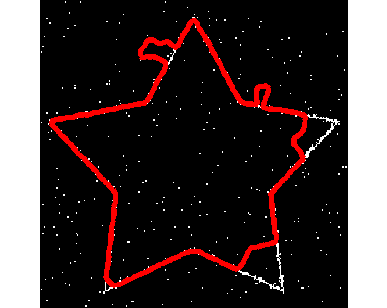
\includegraphics[width=\textwidth]{Chapters/Images/Noise/gvfimp1}
\caption{}
\end{subfigure}
\begin{subfigure}[c]{0.3\linewidth}
\centering
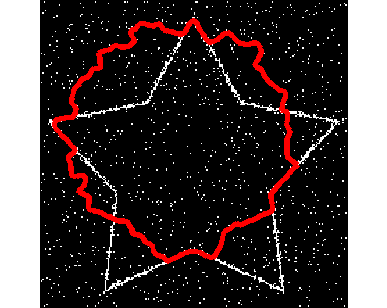
\includegraphics[width=\textwidth]{Chapters/Images/Noise/gvfimp5}
\caption{}
\end{subfigure}
\begin{subfigure}[c]{0.3\linewidth}
\centering
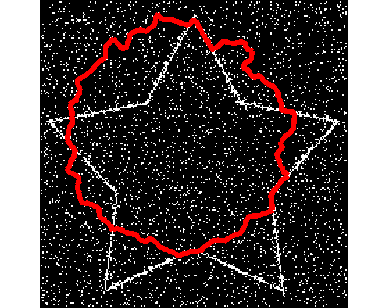
\includegraphics[width=\textwidth]{Chapters/Images/Noise/gvfimp15}
\caption{}
\end{subfigure}
\caption{GVF à 100 itérations sur une image bruitée par un bruit impulsionnel pour (a) $1\%$,(b) $5\%$,(c) $15\%$ de pixels touchés}
\end{figure}

\begin{figure}[H]
\centering
\begin{subfigure}[c]{0.3\linewidth}
\centering
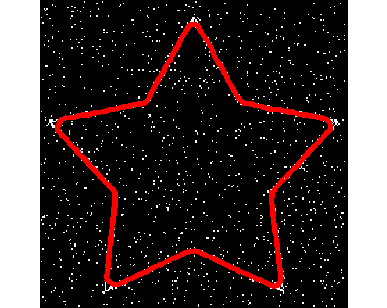
\includegraphics[width=\textwidth]{Chapters/Images/Noise/vfcimp5}
\caption{}
\end{subfigure}
\begin{subfigure}[c]{0.3\linewidth}
\centering
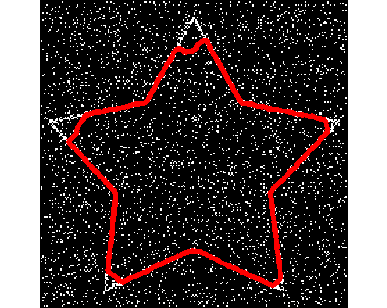
\includegraphics[width=\textwidth]{Chapters/Images/Noise/vfcimp15}
\caption{}
\end{subfigure}
\caption{VFC à 100 itérations sur une image bruitée par un bruit impulsionnel pour (a) $5\%$,(b) $15\%$ de pixels touchés}
\end{figure}

\begin{figure}[H]
\centering
\begin{subfigure}[c]{0.3\linewidth}
\centering
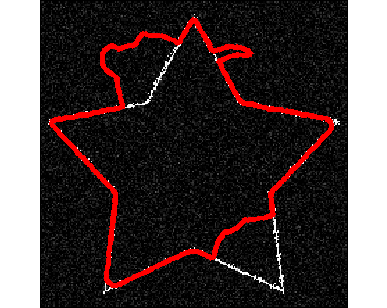
\includegraphics[width=\textwidth]{Chapters/Images/Noise/gvfg1}
\caption{}
\end{subfigure}
\begin{subfigure}[c]{0.3\linewidth}
\centering
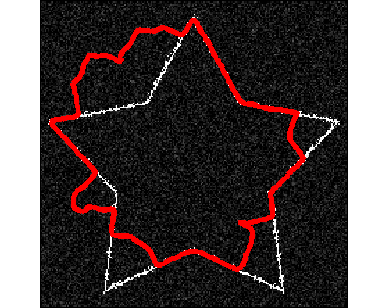
\includegraphics[width=\textwidth]{Chapters/Images/Noise/gvfg5}
\caption{}
\end{subfigure}
\begin{subfigure}[c]{0.3\linewidth}
\centering
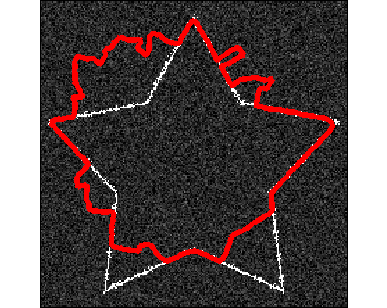
\includegraphics[width=\textwidth]{Chapters/Images/Noise/gvfg15}
\caption{}
\end{subfigure}
\caption{GVF à 100 itérations pour une image bruitée par un bruit additif gaussien pour (a) $\sigma = 0.01$,(b) $\sigma = 0.05$,(c) $\sigma = 0.15$}
\end{figure}

\begin{figure}[H]
\centering
\begin{subfigure}[c]{0.3\linewidth}
\centering
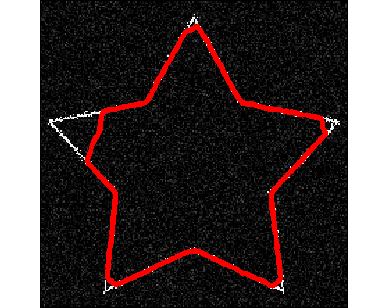
\includegraphics[width=\textwidth]{Chapters/Images/Noise/vfcg1}
\caption{}
\end{subfigure}
\begin{subfigure}[c]{0.3\linewidth}
\centering
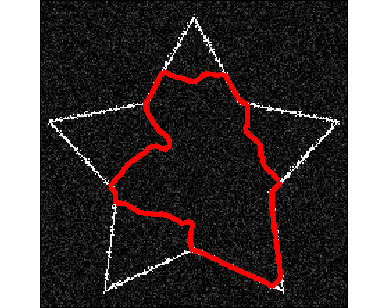
\includegraphics[width=\textwidth]{Chapters/Images/Noise/vfcg5}
\caption{}
\end{subfigure}
\\
\begin{subfigure}[c]{0.3\linewidth}
\centering
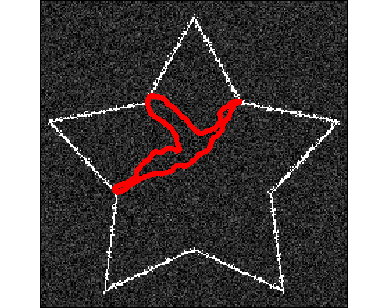
\includegraphics[width=\textwidth]{Chapters/Images/Noise/vfcg15}
\caption{}
\end{subfigure}
\begin{subfigure}[c]{0.3\linewidth}
\centering
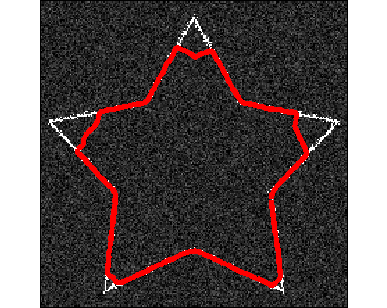
\includegraphics[width=\textwidth]{Chapters/Images/Noise/vfcsmallkernel}
\caption{}
\end{subfigure}
\caption{VFC à 100 itérations pour une image bruitée par un bruit additif gaussien pour (a) $\sigma = 0.01$,(b) $\sigma = 0.05$,(c) $\sigma = 0.15$. (d) VFC à 100 itérations pour une image bruitée par un bruit additif gaussien $\sigma=0.15$ avec une taille de noyau $R=64$}
\end{figure}

